\documentclass{beamer}

% fonts and text
\usepackage[utf8]{inputenc}
\usepackage[T1]{fontenc}

% graphics
\usepackage{graphicx}
\usepackage{tikz}
\usetikzlibrary{positioning}
\usetikzlibrary{matrix}

% math
\usepackage{mathtools}

% source code
% to use minted, you need to install `pygments` python package
% on some platforms, `pygmentize` executable is separate from `pygments` package
% for more info, see minted docs or test your google skills
% \usepackage[cache=false]{minted}

\usetheme{ltml}

\title[Short Title]{Title of Your Presentation}
\author{Your Name}
\date{18. 10. 2018}

\begin{document}

\frame[plain, noframenumbering]{\titlepage}

\begin{frame}
  \frametitle{Frame Title}

  Content

  \begin{itemize}
    \item List support
  \end{itemize}

  \begin{figure}
      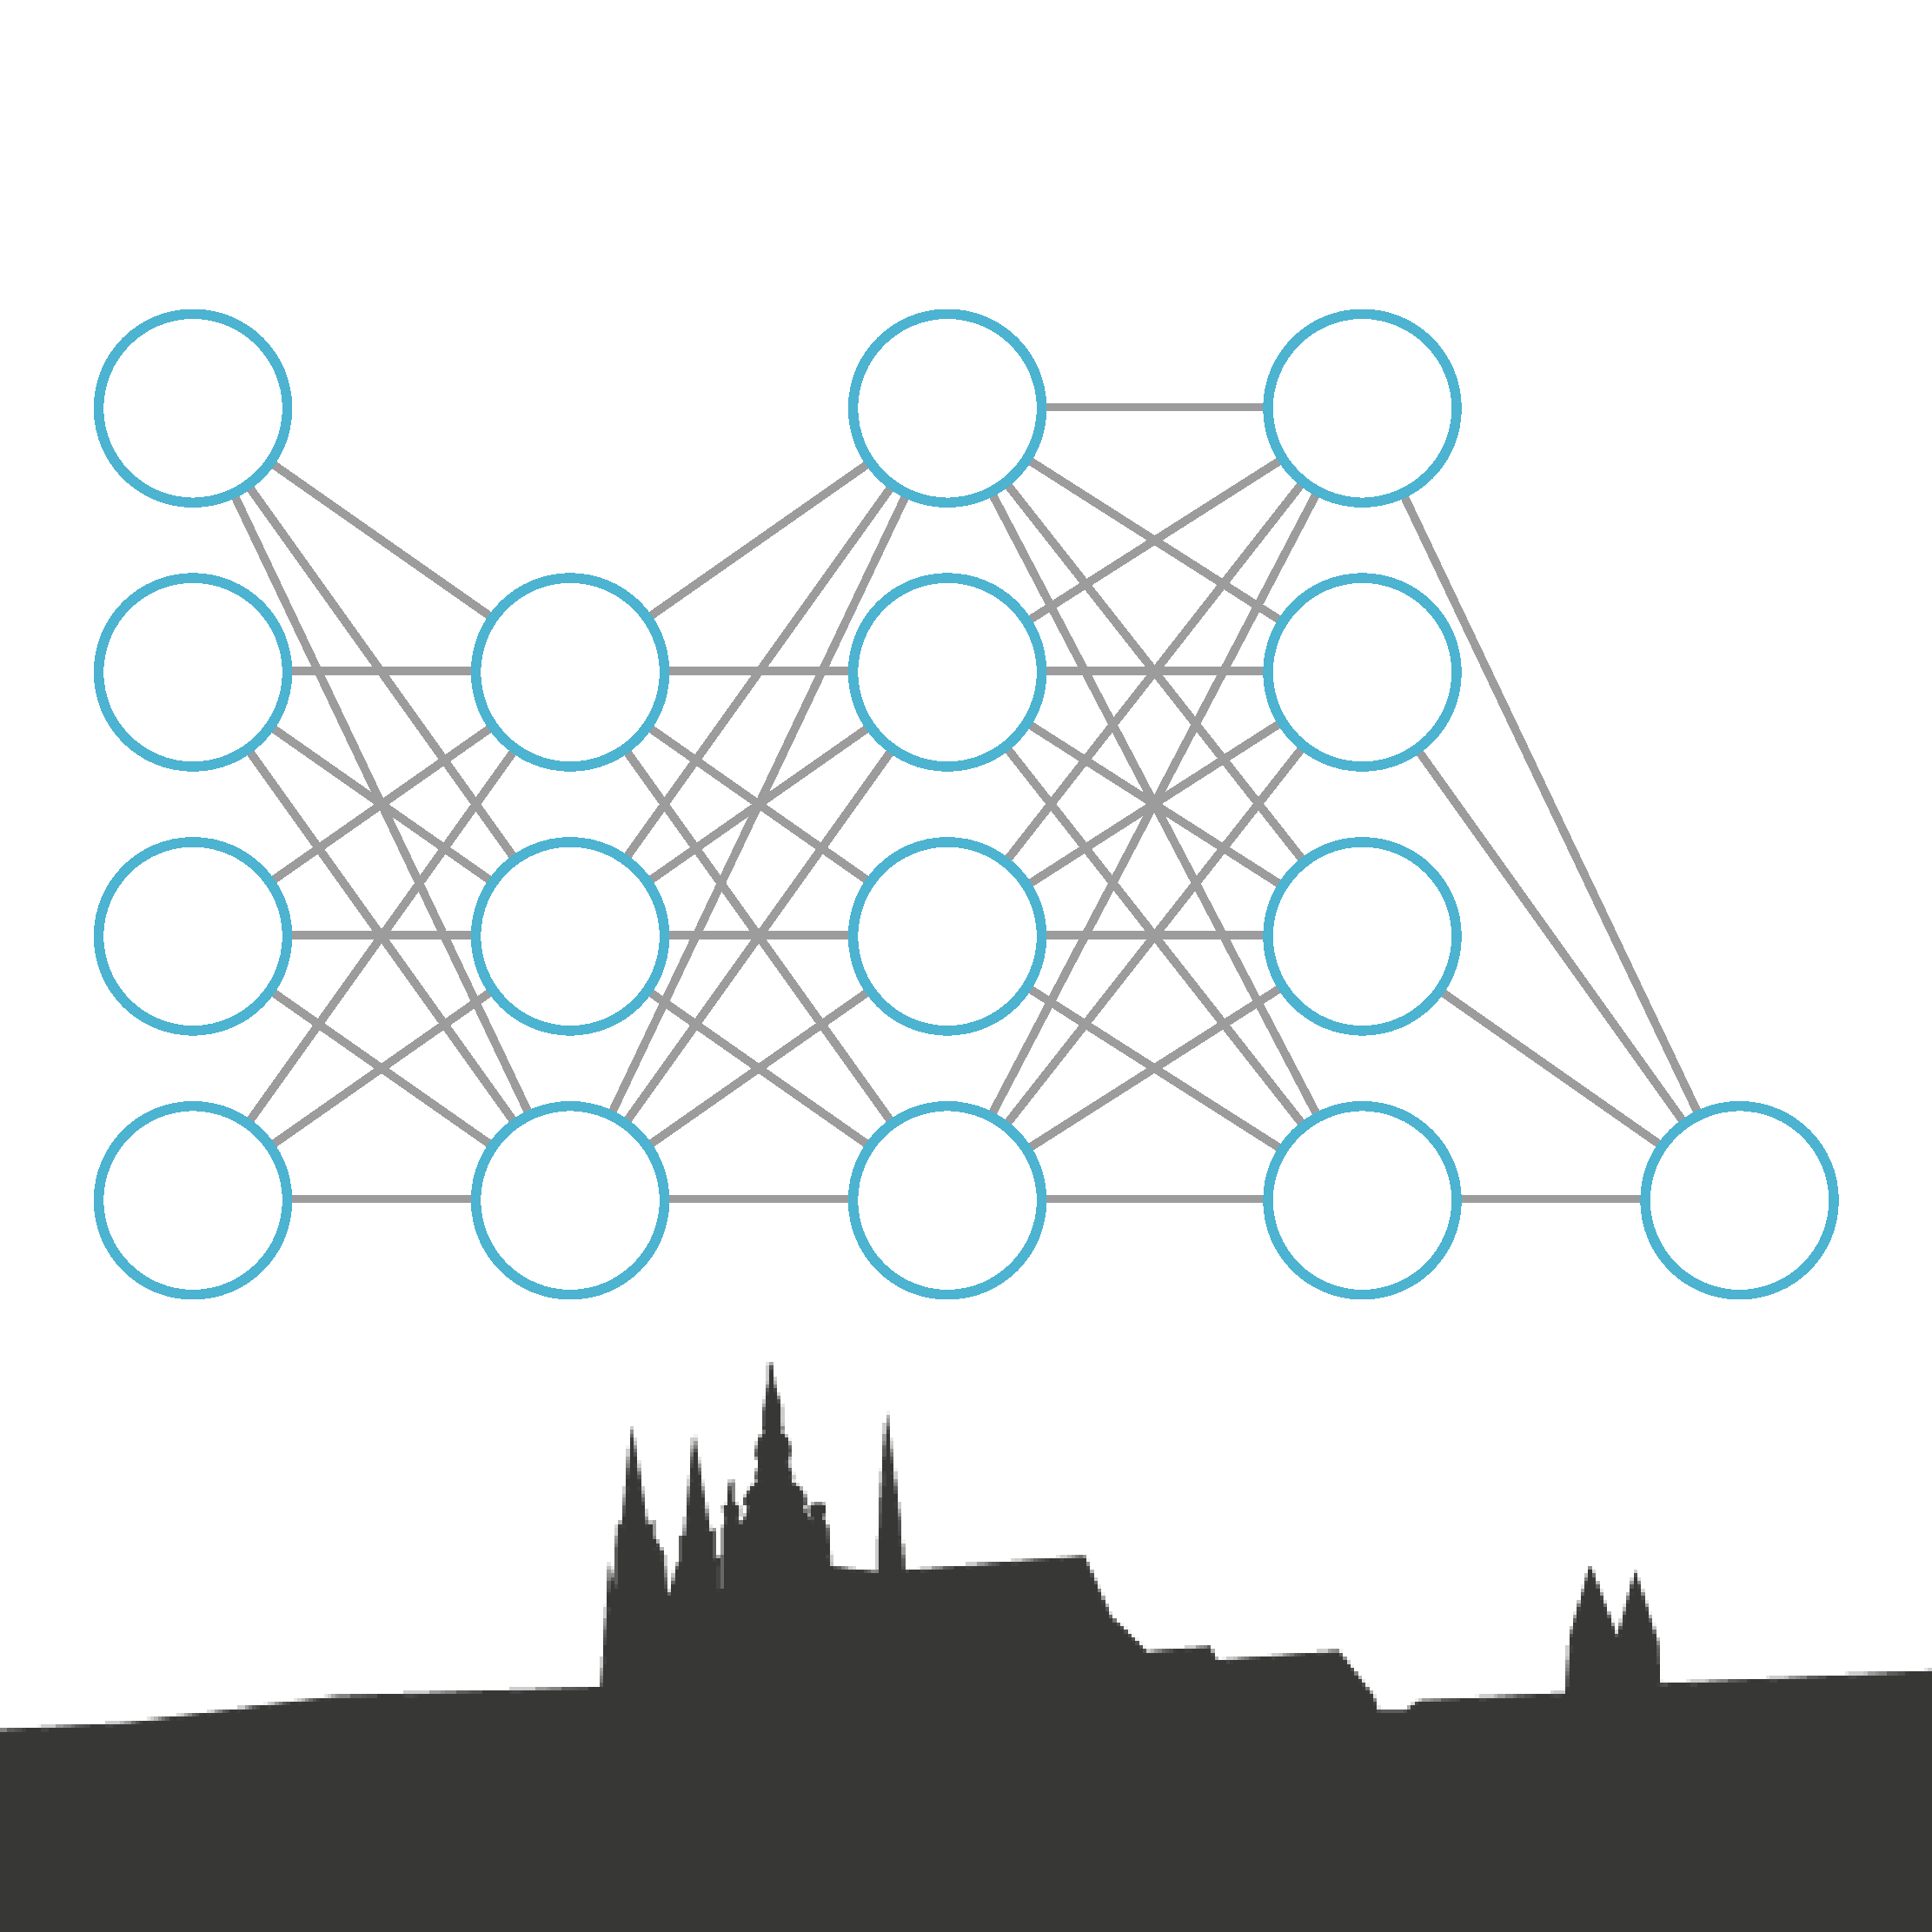
\includegraphics[width=0.4\textwidth]{logo}
      \caption{This is our logo}
      \label{fig:logo}
  \end{figure}

\end{frame}

\begin{frame}
  \frametitle{Mathematics}

  \begin{equation*}
    (a + b)^2 = a^2 + 2ab + b^2
  \end{equation*}

\end{frame}

% \begin{frame}[fragile]
%   \frametitle{Source Code}
%
%   \begin{minted}{python}
%
% def hello(name):
%     print('Hello, {}!'.format(name))
%
%   \end{minted}
%
% \end{frame}

\begin{frame}
  \frametitle{Very Long Heading Which Would Obviously Overlap}

  \begin{itemize}
    \item Template handles longer headings and automatically resizes their size
    \item If the heading overlaps even after that, consider if it is a proper heading
  \end{itemize}

\end{frame}

\end{document}
